\documentclass[draftclsnofoot,onecolumn,letterpaper,10pt]{IEEEtran}
\pagestyle{empty}
\usepackage{geometry}
\usepackage{pgfgantt}
\geometry{textheight=9.5in, textwidth=7in}
\usepackage{float}
\usepackage{graphicx}
\usepackage{algorithm2e}
\usepackage{rotating}
\usepackage{listings}
\usepackage{color}
\definecolor{mygreen}{rgb}{0,0.6,0}
\definecolor{mygray}{rgb}{0.5,0.5,0.5}
\definecolor{mymauve}{rgb}{0.58,0,0.82}

\newcommand{\subparagraph}{}
\usepackage{titlesec}
\setcounter{secnumdepth}{4}
\graphicspath{{images/}}
\lstset{%
  backgroundcolor=\color{white},   % choose the background color; you must add \usepackage{color} or \usepackage{xcolor}; should come as last argument
  basicstyle=\footnotesize,        % the size of the fonts that are used for the code
  breakatwhitespace=false,         % sets if automatic breaks should only happen at whitespace
  breaklines=true,                 % sets automatic line breaking
  captionpos=b,                    % sets the caption-position to bottom
  commentstyle=\color{mygreen},    % comment style
  extendedchars=true,              % lets you use non-ASCII characters; for 8-bits encodings only, does not work with UTF-8
  frame=R,	                   % adds a frame around the code
  keepspaces=true,                 % keeps spaces in text, useful for keeping indentation of code (possibly needs columns=flexible)
  keywordstyle=\color{blue},       % keyword style
%  language=Python,                 % the language of the code
  morekeywords={self},           % if you want to add more keywords to the set
  numbers=left,                    % where to put the line-numbers; possible values are (none, left, right)
  numbersep=0em,                   % how far the line-numbers are from the code
  numberstyle=\tiny\color{mygray}, % the style that is used for the line-numbers
  rulecolor=\color{black},         % if not set, the frame-color may be changed on line-breaks within not-black text (e.g. comments (green here))
  showspaces=false,                % show spaces everywhere adding particular underscores; it overrides 'showstringspaces'
  showstringspaces=false,          % underline spaces within strings only
  showtabs=false,                  % show tabs within strings adding particular underscores
  stepnumber=1,                    % the step between two line-numbers. If it's 1, each line will be numbered
  stringstyle=\color{mymauve}     % string literal style
}


\begin{document}
{\centering
	{\scshape\LARGE Oregon State University\par}
	\vspace{1cm}
	{\scshape\Large CS Senior Design Final Report\par}
	\vspace{1.5cm}
	{\huge\bfseries Brew.ai - Team 7\par}
	\vspace{2cm}
	{\Large\itshape Connor Yates\par}
	\texttt{yatesco@oregonstate.edu\\}
	{\Large\itshape Aravind Parasurama\par}
	\texttt{parasura@oregonstate.edu\\}
	{\Large\itshape Cody Holliday\par}
	\texttt{hollidac@oregonstate.edu\\}
	\vspace{2cm}
	\vfill
% Bottom of the page
	{\large \today\par}
}
\newpage
\tableofcontents
\newpage

\section{Introduction}

Who requested it?
Why was it requested?
What is its importance?
Who was/were your client(s)?
Who are the members of your team?
What were their roles?
What was the role of the client(s)? (I.e., did they supervise only, or did they participate in doing development)


\section{Client Requirements}
\documentclass[draftclsnofoot,onecolumn,letterpaper,10pt]{IEEEtran}
\pagestyle{empty}
\usepackage{geometry}
\usepackage{pgfgantt}
\geometry{textheight=9.5in, textwidth=7in}

\author{Connor Yates\\
\texttt{yatesco@oregonstate.edu\\}
\and
Aravind Parasurama\\
\texttt{parasura@oregonstate.edu\\}
\and
Cody Holliday\\
\texttt{hollidac@oregonstate.edu\\}}
\date{\today}
\title{brew.ai Client Requirements}
\begin{document}
\maketitle

\newpage
\tableofcontents
\newpage
\section{Overview}
Section 1A describes the scope of the requirements for the brew.ai project.
Section 2 defines terms used in the document as well as terms that are normally used when discussing the project.
Section 3 Introduces the purpose of this document.
Section 4 outlines the project in a high level.
Section 5 describes the requirements through user stories.

\subsection{Scope}
brew.ai is a device that automatically brews mead or beer, and learns how to brew better over time.
The scope of this document focuses on the specifications of the device as well 
as the steps to build a business around it.

\section{Definitions}
\begin{itemize}
	\item Actuators - Electromechanical devices that allow the microprocessor to 
		affect the fermentation process.
	\item Artificial Intelligence - A learned control policy which controls 
		the microcontroller.
	\item AI - See Artificial Intelligence.
	\item Brewing Setup - The collection of brewing vessels where fermentation 
		occurs.
	\item Microcontroller - A small, simple computer connected to sensors and 
		actuators on the brewing setup.
	\item Sensors - A collection of electronic sensors which measure useful data, 
		such as temperature and specific gravity.
\end{itemize}

\section{Introduction}
Broadly, this document serves to layout the requirements of this project.
These requirements focus on both business and technological aspects.
This document aims to assist in
\begin{itemize}
	\item Providing specific deliverables and deadlines for the developers.
	\item Define the initial scope of the project.
	\item Create a structure to advance the business possibilities of the project.
	\item Incorporating the mindset and wants of the user into the final project.
\end{itemize}
To this end, the document provides an overview of the project, followed by the specific requirements.
The specific requirements will provide context for specific goals, and means by which to 
measure the attainment of the goals.

\section{Overall Description}
\subsection{Product Perspective}
This project is self contained, but it does use other projects to help create it.
TensorFlow is a library created by Google for the development of Artificial Intelligence.
TensorLayer is an extension on top of TensorFlow for Reinforcement Learning extensions.

\subsubsection{User Interfaces}
The Android user interface should be designed per Google material design guidelines.
The Android interface should have two states: pre-brewing and post-brewing.
The pre-brewing interface will allow users to select the taste of their batch.
There will also be a section for advanced settings that allow the user to tune how the
device will function during the brewing process.
The post-brewing interface will have the user rate the batch based on different 
characteristics of the batch as well as a general overall satisfaction with the batch.

\subsubsection{Hardware Interfaces}
The Android software will interact with the brewing hardware through a microcontroller.
The microcontroller will provide the Android software an interface for interacting with 
the brewing hardware; allowing the software both to modify brewing behavior and to gather
telemetry about an ongoing process.

\subsubsection{Memory}
The microcontroller will have limited memory space for instructions and sensory inputs. Any
process of complexity will need to be kept on the Android system or learning service backend.

\subsubsection{Operations}
The device will have three states: pre-brewing, brewing, and post-brewing.
Pre and post brewing are characterized by inputs from the user.
Pre-brewing will take inputs from the user either in a simple or advanced way.
Simple inputs are how the mead should taste, and advanced inputs are technical details on how the device will make the brew.
The brewing state will be the device brewing the mead without input from the user.
During the brewing state the user can cancel the operation.
During the post-brewing state the user will have a menu that will have different sections on different aspects of the flavor.
After completion of the short quiz, these menus will save the data and give it to the AI for analysis.
Ideally data will be saved at every point in the operation so that when the machine is plugged in again, it can prompt the user if it wants to make the batch again or what the user thinks of the previous batch.

\subsubsection{Site Adaptation Requirements}
The brewing device will incorporate sensors and microcontrollers that are effectively housed
in order to prevent any kind of water damage to sensitive parts.

\subsection{Product Functions}
The project will have two functions:
\begin{itemize}
	\item Brew beer or mead
	\item Learn from the user how the previous batch tastes
\end{itemize}

\subsection{User Characteristics}
User experience in the brewing process will range from absolute beginner to experienced brewer.
These characteristics are reflected in the options given in the user interface.

\subsection{Constraints}
\subsubsection{Safety Considerations}
A major consideration for dealing with food or beverages is cleanliness.
This project will incorporate safety measures so that when the device brews a batch it will be safe for human consumption.
The device will have to be safeguarded to prevent injury of the user during operation.
\subsubsection{Hardware Limitations}
The hardware will be inexpensive as well as easy to incorporate into a singular device.
The microcontroller will have to interface well with this device as well as the computer giving it instructions.
The computer will need an interface for the microcontroller as well.
When fully complete the hardware will be both modular and waterproof.

\subsection{Assumptions and Dependencies}
The AI will operate using the TensorFlow libraries designed by Google, and TensorLayer extension libraries for reinforcement learning.

\section{Specific Requirements}
\subsection{Customer User Stories}
\begin{itemize}
	\item Automated brewing will make brewing accessible to even amateurs. For those interested in trying brewing simply as an
		occassional hobby, quality results will be accessible with brew.ai. An easy to set up, fully linked automated brewing system can
		become an integral part of holiday cooking when brewing for the family.
	\item A backend learning service attached to the device can help two classes of consumers. The amateur brewer can utilize this 
		service to effortlessly create simple and unique flavors with beer and mead. The professional brewer can utilize this service
		to better improve recipes that undergo constant revision.
	\item A simple, preprogrammed microcontroller solution for controlling the brewing hardware helps keep the technology out of the way
		of consumers. Having less functionality on the microcontroller removes any necessity of updates on that level, and also makes
		the product more servicable as users can simply swap out hardware devices on their systems.
	\item An Android client provides a friendly and easy to use interface for the consumer. The nature of touch screen interfaces lends 
		itself to an easy to use, but powerful layout. The ability to deliver over the air updates on the fly to Android applications
		allows for functionality to be tweaked after any potential hardware is put into production. The Android client provides simplified
		controls and guided instructions for the amateur brewer to brew with ease. The client also provides more advanced controls for more
		professional brewers with more knowledge of the various factors that go into a brew.
\end{itemize}
\subsection{Technical Requirements}
Based upon our own ideas of for the project, as well as the concepts from the user stories, the technical requirements can be summarized as follows.
These requirements are presented in order of their completion.
I.e., requirements must be completed in their presented order.
\begin{itemize}
	\item Assemble a brewing setup.
	\item Acquire electronics hardware - microcontroller, actuators, and sensors.
	\item Gather data for training machine learning algorithm.
	\item Design learning structure for the control policy.
	\item Create the learning structure and control policy.
	\item Train the policy.
	\item Use the policy to automate the fermentation process.
	\item Create a user interface to monitor and control the brewing process.
\end{itemize}
\begin{ganttchart}{3}{8}
	\gantttitle{2016-2017}{6} \\
	\gantttitlelist{3,...,8}{1} \\
	\ganttgroup{Assemble brewing setup}{3}{6} \\
	\ganttgroup{Build software solution}{6}{8} \\
	\ganttbar{Acquire electronics hardware}{3}{4} \\
	\ganttlinkedbar{Construct brewing hardware}{5}{6} \ganttnewline
	\ganttlinkedmilestone{Hardware complete}{6} \ganttnewline
	\ganttlinkedbar{Build Android client}{5}{7} \ganttnewline
	\ganttlinkedbar{Build learning backend}{6}{8}
\end{ganttchart}
\subsection{Business Requirements}
As we develop this project we must treat it as if we are starting a business.
To go about starting a business we have to go through a series of steps to set it up.
\begin{itemize}
	\item Develop a business plan using the Lean Canvas Model
	\item Interview businesses and homebrewers about their needs as brewers as well as what they want to change about their process.
	\item After developing a prototype, ask businesses and homebrewers about possible features to add to the device.
	\item Make a pitch deck.
	\item Pitch the idea at an event.
	\item Interview with a potential customer.
\end{itemize}
\end{document}

\section{Difference Between Final Product and Client Requirements}
The Client Requirements document was not modified at all during the year, even as we changed the design.
We did however, fail to complete some of the business related requirements from the original document.

\begin{ganttchart}[
    y unit title=0.5cm,
    y unit chart=0.6cm,
    time slot format=isodate-yearmonth,
    compress calendar,
    title/.append style={shape=rectangle, fill=black!10},
    title height=1,
    bar/.append style={fill=green!90},
    bar height=.6,
    bar label font=\normalsize\color{black!50},
    group top shift=.6,
    group height=.3,
    group peaks height=.2,
    bar incomplete/.append style={fill=green!40}
  ]{2016-10-27}{2017-05-02}
  \gantttitlecalendar{year} \\
  \gantttitlecalendar{month} \\
  \ganttbar{Requirements Document}{2016-10-28}{2016-11-04} \\
  \ganttlinkedbar{Survey Potential Users and Customers}{2017-02-17}{2017-02-30} \\
  \ganttlinkedbar{Research AI, ML, RL structures}{2016-11-04}{2016-11-24} \\
  \ganttgroup{Construct Prototype}{2017-01-06}{2016-12-19} \\
    \ganttbar{Hardware}{2016-11-04}{2016-11-05} \\
    \ganttbar{Electronics}{2016-11-05}{2016-11-10} \\
    \ganttlinkedbar{Gather Data}{2016-11-10}{2016-12-05} \\
    \ganttbar{Construct Control Policy}{2016-12-05}{2016-12-19} \\
    \ganttbar{Gather More Data}{2016-12-19}{2017-01-19} \\
  \ganttgroup{Second Prototype Iteration}{2017-01-19}{2017-03-04} \\
    \ganttbar{Assemble Hardware}{2017-01-20}{2017-01-21} \\
    \ganttlinkedbar{Electronics}{2017-01-21}{2017-01-26} \\
    \ganttbar{Gather Data}{2017-01-26}{2017-02-19} \\
    \ganttbar{Rework Control Policy}{2017-02-19}{2017-03-14} \\
    \ganttbar{Prepare For Expo}{2017-03-14}{2017-04-29}
\end{ganttchart}

\begin{center}
\begin{tabular}{ lll p{0.3\linewidth} }
 \# & Requirement & What happened to it? & Comments \\
\hline
 1 & Microcontroller & Deemed unnecessary and removed from design. & Actuators and sensors  were integrated directly into the Raspberry Pi \\ 
 2 & Business Requirements & Incomplete. & Only the interviews were conducted. \\  
\end{tabular}
\end{center}



\section{Design Document}
\documentclass[draftclsnofoot,onecolumn,letterpaper,10pt]{IEEEtran}
\pagestyle{empty}
\usepackage{geometry}
\geometry{textheight=9.5in, textwidth=7in}

\usepackage{float}
\usepackage{graphicx}
\usepackage{algorithm2e}
\usepackage{pgfgantt}

\newcommand{\subparagraph}{}
\usepackage{titlesec}

\titleformat{\section}[block]{\bfseries\Large}{\thesection}{0.4em}{}
\titleformat{\subsection}[block]{\bfseries\large}{\thesubsection}{0.4em}{}
\titleformat{\subsubsection}[block]{\bfseries\normalsize}{\thesubsubsection}{0.4em}{}
\setlength{\parindent}{0pt}
\renewcommand{\thesection}{\arabic{section}}
\renewcommand{\thesubsection}{\thesection.\arabic{subsection}}
\renewcommand{\thesubsubsection}{\thesubsection.\arabic{subsubsection}}



\date{\today}

\title{brew.ai Design Document}

\begin{document}
{\huge\textbf{Senior Software Engineering Design Group 7}}
	\vspace{1cm}

{\Huge\textbf{brew.ai Design Document}}

\vspace{2cm}
\textbf{Connor Yates} yatesco@oregonstate.edu

\textbf{Aravind Parasurama} parasura@oregonstate.edu

\textbf{Cody Holliday} hollidac@oregonstate.edu

\vspace{2cm}
\textbf{Sponsor}

Dale McCauley, College of Business, Oregon State University

\vspace{0.5cm}
	\textbf{Approved:} 

	\textbf{Version:} 1.0


\newpage
\begin{abstract}
	Home beer or mead brewing is not currently a process as simple as brewing coffee.
	We aim to change this, and make home brewing as easy as brewing coffee with the OpenBrew project.
	The OpenBrew project will consist of two major components:
	A hardware system for physically automating the brewing process, and a software system for managing the brewing process, utilizing machine learning 
		to optimize mead or beer recipes.
	Through these components, a user will be able to easily incorporate a fully automated, intelligent home brewing system into an existing setup or 
		as the framework to construct a new brewing system.
\end{abstract}
\newpage
\tableofcontents
\newpage
\section{Introduction}
% Perhaps get rid of these subsection titles, and just combine it into one larger section with appropriate paragraph spacings.
% These talk about the Purpose, scope, etc, of this paper.
brew.ai is a hardware and software solution for automated brewing of mead or beer. Currently, home brewing requires a lot of time, knowledge, and 
	patience. 
As such, it is not accessible to amateurs, and brew.ai attempts to solve this problem. 
From amateurs to professional brewers, we want brew.ai to be useful in automating the brewing process, and helping brewers make better tasting products. 
The brew.ai device itself is a bucket lid that will fit over a brewing device and have various modules incorporated in it. 
The lid device will monitor and control temperature, send and receive commands/data to and from the Android application, and monitor fermentation status.
Improving recipes will take place in the back-end, in the form of a service that the Android software will communicate with. 
As a user, setup will simple and essentially plug-and-play. 
No technical knowledge is needed beyond knowing how to pair a bluetooth bucket lid with an Android device.

\subsection{Purpose}
This document describes the architecture and design of the brew.ai project.
It conforms to the IEEE 1016 System Design Document specification, and lays out the design of hardware, learning, and android interfaces for the project.
By following the designs presented in this document, a technically skilled person or team of people will be able to replicate the prototype we will produce.

\subsection{Scope}
Stated generally, brew.ai is a device which automatically brews fermented drinks and improves its performance over time based on user feedback.
This allows for users who are inexperienced with automated control systems or home brewing to create their own home-brewed fermented drinks.
While brew.ai mainly focuses on home brewing applications, it can theoretically scale to larger applications.

\subsection{Document Overview}
This document is split into three major sections.
The first two talk about the project on a high level, describing who will use the product, what they can do and why they would want to accomplish a goal, and how the system will allow the user to accomplish their goal.
The third major section contains technical design information, to be used by developers to implement the brew.ai prototype.


\section{Glossary}

\section{Stakeholders and Design Concerns}
% Here we list out the design concerns of stakeholders (users, etc...) that we address in this document.
% By laying out the design concerns now, we can address each in turn in the subsequent design sections.
While the design team and sponsor are direct stakeholders of this project, they do not have any concerns, apart from technological feasibility, that impact the design of the product.
Rather, the eventual users are the stakeholders whose requirements influence the final design of the product.

There are three major design concerns when viewing this product from the viewpoint of the user.
First, the brewing system must be able to learn from past trials, based on user feedback. 
This design concern is addressed in Section~\ref{sec:learning}.
Secondly, the system must automate the brewing process. 
This design concern is addressed in Section~\ref{sec:hardware}.
Finally, the user must have a method of interacting with the brewing device, to measure progress and see how the system is performing.
This is addressed in Section~\ref{sec:android}.
While these design concerns are broad, when put together they describe the basis of the project.

\section{System Overview}
In order to satisfy the three major design concerns, this project is cleanly divided into three respective technological sections.
These technological sections are self-contained, except for data messages which must be shared intermittently.
This section provides a brief overview of these sections, and describes the method by which they will communicate.

To implement the intelligent learning, a standard reinforcement learning agent will be created, and will be able to communicate with both sections.
Hardware will be created to solve the task of automated brewing, and will communicate exclusively with the intelligent agent.
A user interface will be created on an dedicated platform, which will communicate with the intelligent agent.
In this design, the intelligent agent can act as the translator between the hardware and user interface.

\subsection{Data Design}
The messages passed between the hardware, agent, and interface are described in this section.
All three sections must be able to transmit and receive specific message types.
The hardware must continually pass current sensor readings to the intelligent agent.
These sensor readings will be communicated as a byte stream, since they are nothing more complicated than a few numbers.
The hardware must be able to receive action requests from the agent.
Action requests will be sent as a status number, signifying which of the three actions described in Section~\ref{sec:learning} the hardware should take.
The user interface will need to communicate basic user requests to the intelligent agent.
Some of these requests, such as an emergency stop, will not take part in the learning process.
Rather, they are passed to the agent module because it already contains this level of functionality, as seen in Section~\ref{sec:learning}.
The user interface will also need to communicate the user's satisfaction to the learning agent.
This message will take part in the learning process, but is not necessary for the learning agent to have until after the batch is completed.
Finally, the user interface needs to receive the current status of the brewing process.
This information, which encompasses elements such as runtime, temperature, and estimated completion time, will be sent in the JSON format.

The dataflow diagram in Figure~\ref{fig:dataflow} summarizes the internal message passing in the brewing system.
\begin{figure}[h]
\begin{center}
	\caption{Dataflow Between the Three Major Components \label{fig:dataflow}}
	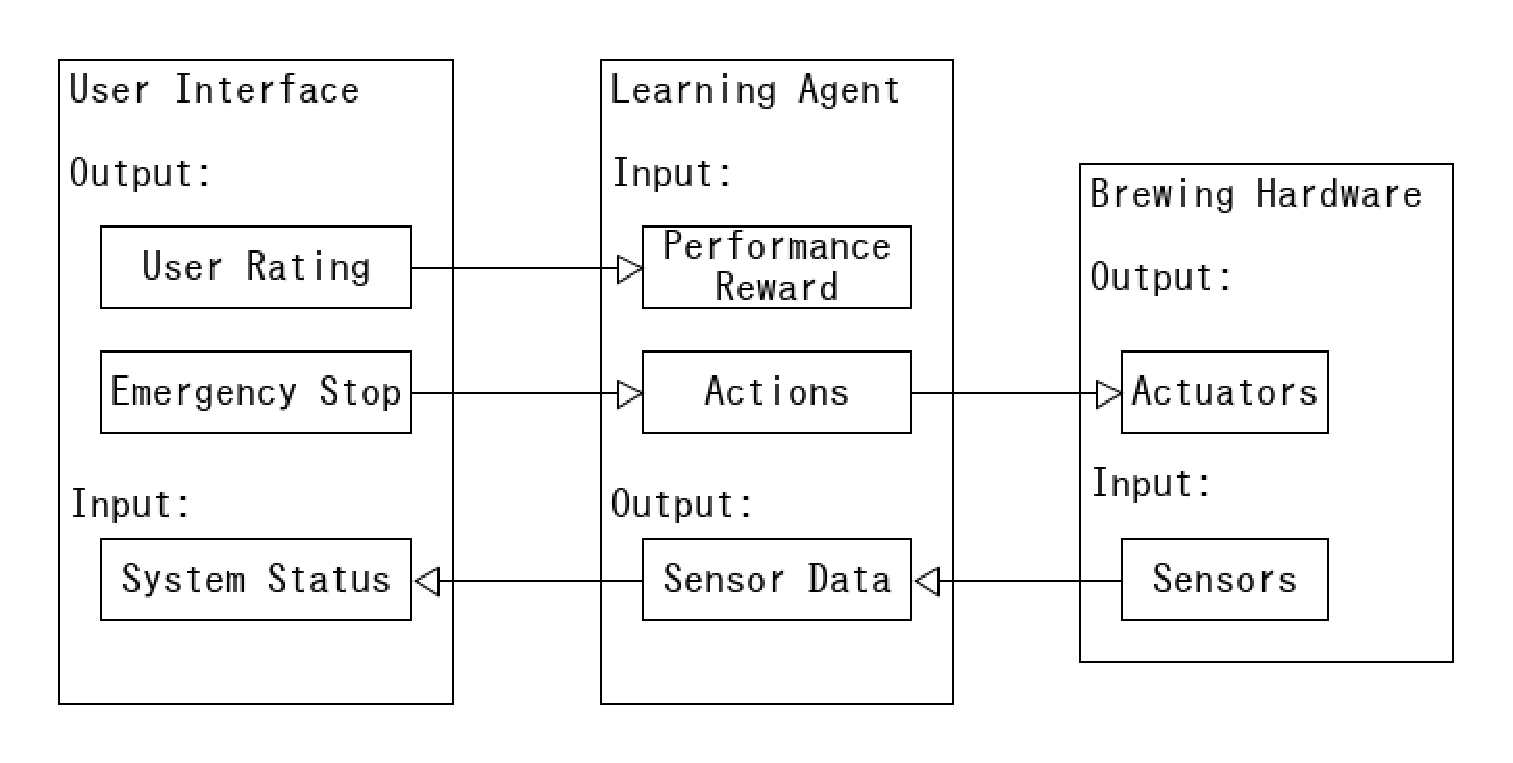
\includegraphics[width=\linewidth]{dataflow.eps}
\end{center}
\end{figure}

\section{Design Viewpoints}
% Details each design point we choose for this project.
% The tech review had 3 technologies, with 3 choices/investigations for each tech.
% Each of the three technologies chosen should be designed in detail in its own "viewpoint".
% each viewpoint then has its own "view". There can be more than one of these.
% the views describe the specific implementations that each viewpoint covers. Refer to the doc for more info.

\subsection{Abstract Learning from Previous Trials}\label{sec:learning}%connor's
From the inception, a major component of this project is the idea that it can learn from mistakes and experiments, and improve the quality of the brew over time.
This section looks at the system design from the viewpoint of artificial intelligence creation.
From this perspective, all other design choices of the project are abstracted into general data sources and sinks.
To further illustrate this point, the view Impact on Other Designs, in Section~\ref{sec:AIImpact}, will introduce the reader to this viewpoint by describing its view of the rest of the system.
From there, the AI system's internal view of the brew.ai system will be explained and designed.

\subsubsection{Impact on Other Designs}\label{sec:AIImpact}
From the viewpoint of learning, the two other major viewpoints, electronic hardware and user interfaces, have little to no impact upon the operations of the system.
There will be interaction between these viewpoints, but that does not imply the other sections will autonomously impact the operation of the system.

From the AI perspective, the system is built as a thinking agent, with the ability to send and receive signals.
This allows the agent to change the world it sees (input signals) through its actions (sent signals).
The hardware will be the main component the AI will interact with, as it provides information about the world through sensors, and can change the world through its actuators.
From this perspective, the hardware is generalized into the two categories: sensors and actuators.
This is a common view for an agent to take in regards to its interaction with the world~\cite{RussellNorvig}.
A diagram summarizing the agent's view of the system is presented in Figure~\ref{fig:AIsystemDesign}.

\begin{figure}[h]\begin{center}
	\caption{brew.ai System Hierarchy from the viewpoint of the agent \label{fig:AIsystemDesign}}
	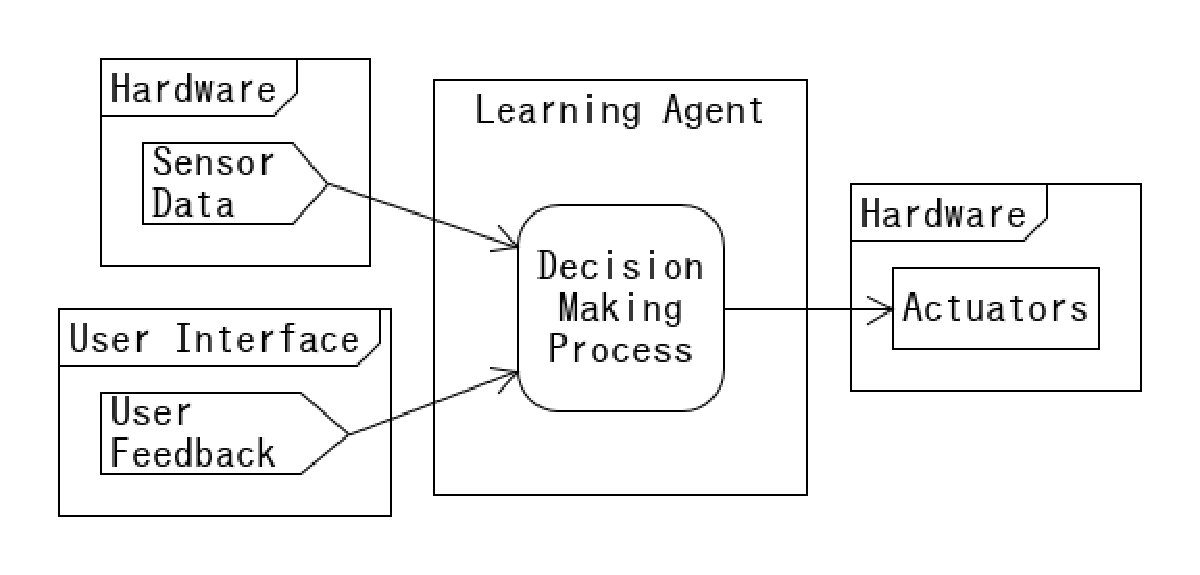
\includegraphics[height=18em]{highView.eps}
\end{center}
\end{figure}

The agent will also view the user interface as source of actuators and sensors, but this will be limited in scope.
The main task of the agent is to brew drinks, not report information to the user.
Therefore, the main decision-making processes will focus on the hardware interaction (reading sensor values, changing temperature levels, etc.) and not on intelligent interaction with the user.
The direct interaction between the user and the AI will be limited to sending statistical information for display, and basic controls such as start-stop controls.

A standard communication layer will be necessary to communicate between the AI, hardware, and interface.
This will be implemented with standard protocols and library packages, such as JSON for interface communication, and byte streams for hardware interaction.
Builtin Python libraries exist for these communication protocols, and subsequently will be used.

\subsubsection{Learning Algorithm} 
% talk about what algorithm I chose.
% Any design considerations that this algorithm requires
% design of this piece, in the context of the project
The agent will be using standard Q-learning, as it provides a proven framework for creating intelligent agents that can learn with delayed rewards~\cite{SuttonBarto}.
This is applicable to our problem since the main reward signal (the input from the user) is not available until the brewing process is complete.

The standard Q-learning algorithm requires a set of states $S$ and a set of available actions $A$.
By performing an action $a_t$ from $A$, the agent is able to change the current state $s_t$.
The Q-table comes into play by learning which action is the best action to take when the agent is in state $s_t$~\cite{SuttonBarto}
The central idea of the algorithm is the value iteration update, defined in Equation~\ref{eq:Q(s,a)}
\begin{equation}\label{eq:Q(s,a)}
	Q(s_t,a_t) \leftarrow Q(s_t, a_t) + \alpha \cdot \left( r_{t+1} + \gamma \cdot \max_a Q(s_{t+1},a) - Q(s_t,a_t) \right)
\end{equation}

Any given state $s_t$ will be composed of the following information:
\begin{itemize}
	\item A numerical signal from the thermocouple
	\item A numerical signal from the carbon dioxide sensor
	\item A numerical signal from the digital hydrometer
	\item A numerical signal representing the current runtime of the brewing process
\end{itemize}
The first three signals come from sensors present in the brewing setup, which will allow the agent to perceive how the current brewing process is proceeding.
The last signal will help the agent differentiate between the start and end of the brewing process, to help differentiate between potentially similar looking states which may require different responses.
The state will be composed as a linear array of this information.
At time $t$, the state $s_t$ will be defined as
\begin{equation}
	s_t = \langle T_t, C_t, G_t, t \rangle
\end{equation}
The units and order of magnitude of the first three signals will be kept at the sensor defaults.
The time dimension will be provided in hours, represented as a floating point number to allow for sub-hour accuracy.

There are three available actions for the agent to choose from.
Two are based on actuators in the brewing setup.
These actuators are a submersible heating element, and a motor controlled stirring mechanism.
The agent can control the power state of the heating element, and the power state of the electric stirrer.
Additionally, the agent can take an action to signal that the brewing process has completed, bringing the process to an end.

\subsubsection{Decision Making Structures}
An important aspect of intelligent decision making is the computational structure which allows for decisions to be made.
Neural networks are a classic method of non-linear function approximation~\cite{RussellNorvig},  which we will use to approximate the Q-table.
This can be done by collapsing the state into a single dimensional vector, and using this as the input to the neural net.
The neural net will output the Q-value associated with each action for this state, which are used by the Q-learning as normal, if they came from a Q-table.

The neural network will take as input the state $s_t$, and output Q values for each associated action.
It will have at least 1 hidden layer residing between the input and output layers.
An example neural net structure is given in Figure~\ref{fig:nn}.

\begin{figure}[h]
\begin{center}
	\caption{Proposed Neural Network Structures \label{fig:nn}}
	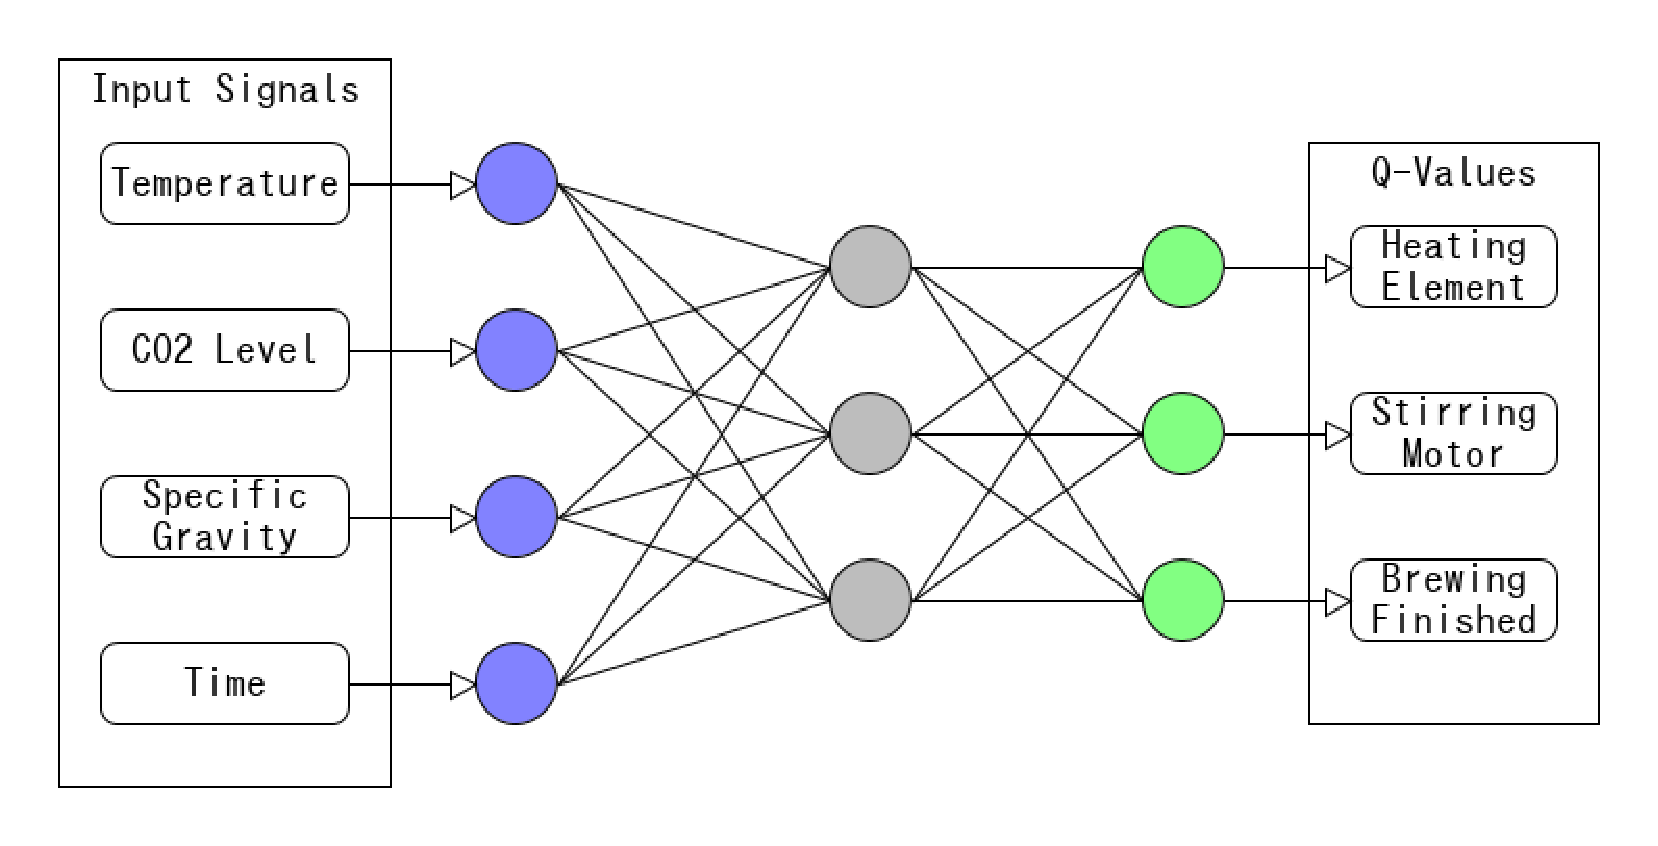
\includegraphics[width=\linewidth]{nn.eps}
\end{center}
\end{figure}

In order to train the neural network to approximate the Q-table, backpropagation will be used along with a sum-of-squares loss function.
Methods such as backpropogation are standard entries in neural-network and machine learning libraries, which we will use to provide the implementation.

If the neural network structure does not provide reliable performance, then we will use a traditional Q-table to implement the learning.
The reason this is not used by default is because we have a continuous state space, which cannot be contained in a finite table.
However, by observing the incoming data, we can provide an encoding scheme which will map the continuous domain of data inputs into a finite, discrete set which can be used to construct the table.

\subsubsection{Overall Agent Structure}
Combining the ideas from the previous sections, the learning agent is summarized as follows, both in diagram and paragraph.

\begin{figure}[h]
\begin{center}
	\caption{Agent structure, showing learning functions, neural network, and data insertion points \label{fig:AgentStructure}}
	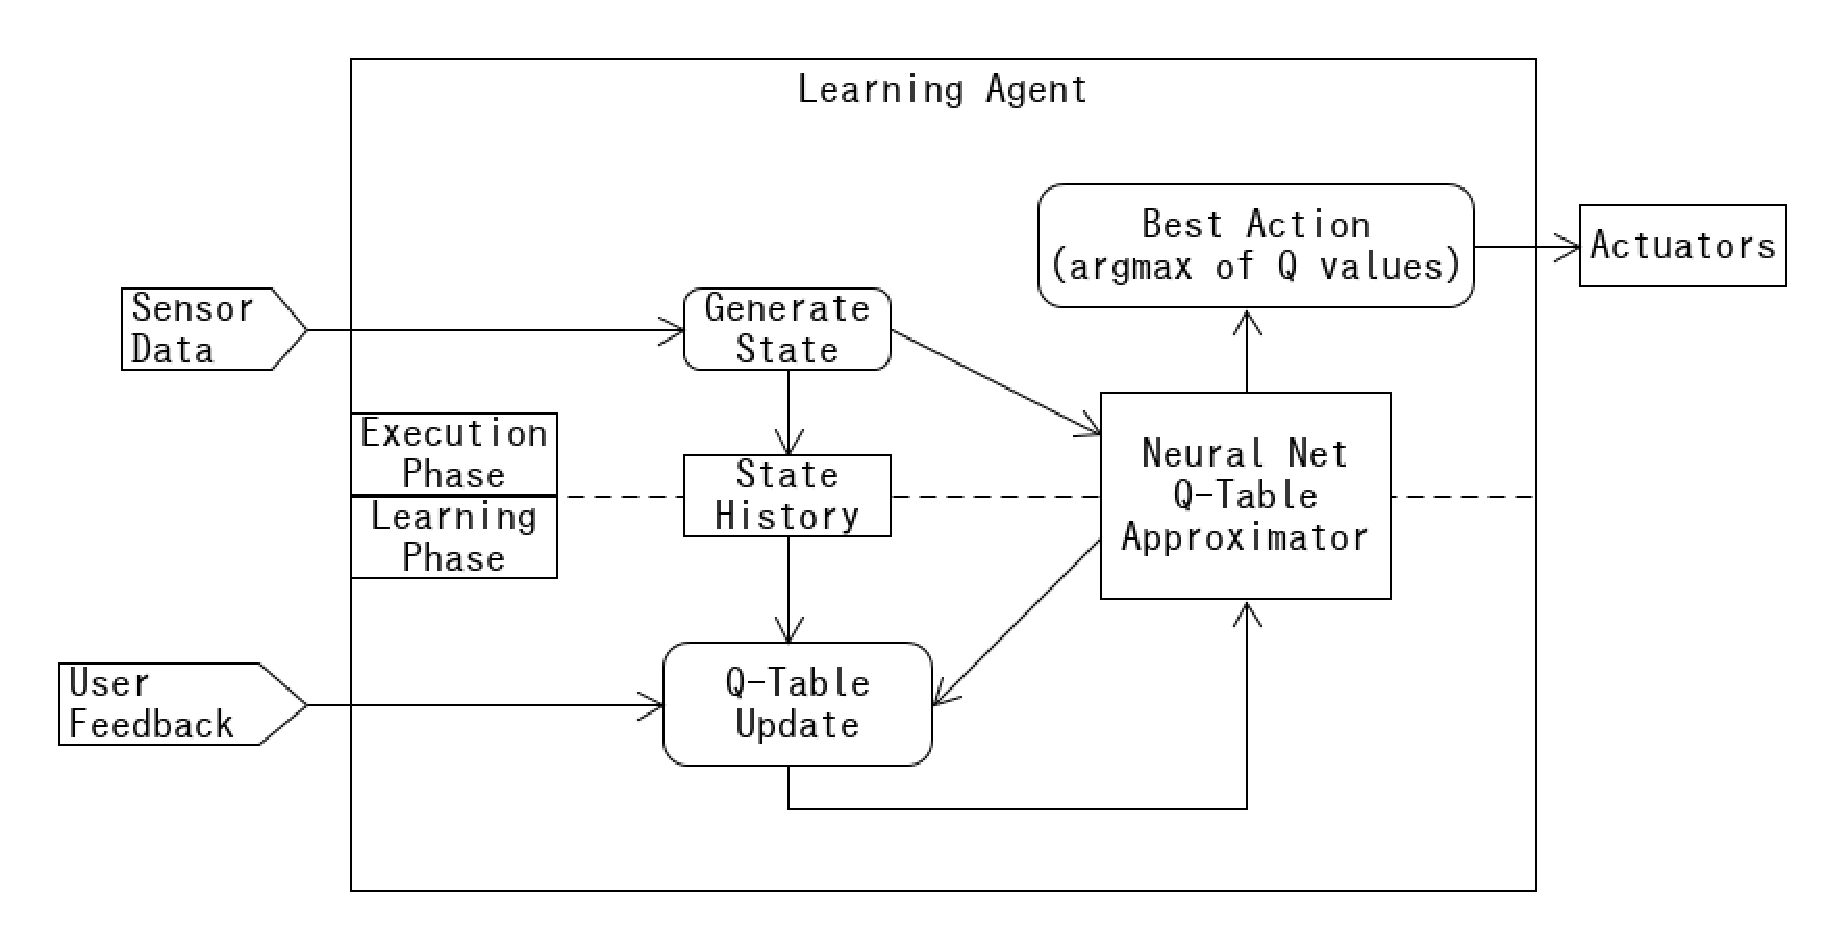
\includegraphics[width=\linewidth]{totalagent.eps}
\end{center}
\end{figure}

A neural network, composed of an 4-dimensional input layer, one or more hidden layers, and a 3 dimensional output layer, will be used as the approximate Q-table.
Input signals will be generated by the microcontroller in direct control of the brewing setup, and combined into the state the agent perceives.
The agent will take actions by taking the action associated with the maximum Q-value at time-step $t$.
These actions will be sent to the microcontroller, where they will be used to control the state of the brewing process.
It will learn by using the Q-learning iterative update function (Equation~\ref{eq:Q(s,a)}), and receiving its reward from the user.


\subsection{Android-Based User Interface Design}\label{sec:android}%cody's
\subsubsection{Interface Device}
The device chosen for the user interface was the Android device.
Android has a well-used set of tools and a huge community for development, which is why it is the best choice.
IDEs like Android Studio are continuously developed to support third party development \cite{AndroidStudio}.
In addition, Android devices can be found at a reasonable price.
The average Android device in 2014 was around \$250 \cite{AndroidStats}, but the Blu Stduio X8 HD is available for \$49.99 as of November 30, 2016 \cite{BluStudioX8}.
The screen is 5 inches from corner to corner, which provides enough space to have many options or buttons on screen.
Our choices are not limited to one device, since there are many other phone manufacturers that produce Android devices.

Choosing the Android as the user interface device determines how the interface is implemented.
Android uses XML for the design and Java for functionality.
Other options are available for programming an Android App, but they are mostly for developing videogames \cite{Pygame}.
Our goals only involve a simple button interface as well as graphical display of data.
Android also offers special libraries that enable native graphing on the device. 
The choice of interface device also affects how the Controller interacts with the interface.
Rather than just being a display for the controller, the Android will have to implement protocol to interact with the controller so that there is a logical flow of data and control.
The data flow between the Android and the controller will be implemented using a TCP connection rather than designing our own message protocol.

\subsubsection{UI Connection to controller}
A USB connection to the controller was determined as the best option for this project.
A simple method of interfacing the Android to the controller is using an Android Debug Bridge \cite{ADBDOCS}.
The Android Debug Bridge is a program that  allows an Android device to be controlled via the command line.
The command line tool allows a PC to manage app installation and activity, as well as file transfers to the device from the PC.
ADB can be installed on a Raspberry Pi, so there are no inherent issues with compatibility \cite{ADBPI}.
To transfer data from the controller to the Android, the controller can just use the ADB command line tool to send the data as a file to the device.
The ADB also allows for port forwarding, so the Android device will communicate with the controller via a TCP connection.
The simplicity of this interface allows for more complex control mechanisms between the controller and the interface as well as leaves room for design improvements.

The controller will have a Python program running that will interact with the Android device using a combination of sockets and bash scripts.
The sockets will be used for control mechanisms, such as starting the brewing process, and the bash scripts will be used as a method for sending data.
Data from a batch is sent from the controller to the Android as a file so that the Android can graph the data locally.
The commands to send the data will live in bash scripts that will be called by the Python program.
Any images that need to be generated on the controller can be sent to the Android via ADB as well.
Physical advantages of a USB connection include preventing loss of data due to interference or connection issues as well as reduce the number of connections on the power supply.


\subsubsection{Dataflow to UI}
The path the data will take is through the controller to the user interface for analysis.
The interface will receive a copy of the data after it is sent to the controller from the microcontroller.
The controller will format the data into a JSON file using the built in JSON Python library \cite{JSONPython}.
The controller will send a JSON file of the data view the ADB command line interface.
After the user interface receives the data, it will turn the JSON file into an object that it will then use to graph the data.
The analysis will take place in the Android app and take place in an asynchronous thread, to prevent the main thread from locking up the interface.
The thread will use a library called Graphview to graph the data on the device. \cite{Graphview}

Graphing on the Android device will reduce the amount of processing that takes place on the controller.
The processing on the controller should be limited to reinforcement learning and data transfer.
However, data transfer and analysis will not take place at the same time on the controller, so there is not a problem with resource sharing, but there is a worry of long term wear and tear.
The brewing device is a long term solution to the homebrewing problem, so we need to maximize the life of the device.
To prevent premature loss of a CPU, the processing load will be spread out over both the controller and the user interface device.

\subsection{Brewing Hardware and Electronic Controls}\label{sec:hardware}%aravind's section
The brewing hardware is expected to perform the commands received from the Android client, while also automatically managing
some basic regulation functions on its own. The hardware will collect data about the brewing process and relay that back to the
Android application.

\subsubsection{Temperature control implementations}
For temperature control, an electric immersion heater will be used.
Immersion heaters are ideal as they can hang from the lid assembly and by submerged into the water. \cite{immersion}
These heaters will provide quick and reliable heating for large quantities of liquid, and this functionality is exactly what is needed for this purpose.
The immersion heater will need to be powered externally to the microcontroller, however control signals for the device must come from the
	microcontroller.
Some kind of power supply or H-BRIDGE module may need to be built to facilitate the power of an immersion heater.

\subsubsection{Data collection from brewing process}
For data collection, an array of sensors has been chosen:
\begin{enumerate}
	\item A thermocouple, for minimal calibration temperature data gathering \cite{thermocouple}. Thermocouples are advantageous over other 
		temperature modules as these are more accurate, and require no tuning with the microcontroller's ADC.
	\item A carbon dioxide sensor, for measuring current fermentation levels by performing calculations versus the initial gravity.
	\item A digital hydrometer for measuring initial gravity \cite{makingmead}.
\end{enumerate}
\subsubsection{Hardware connection to the client}
Data will be transmitted to the front-end by means of bluetooth. A bluetooth module will be used that supports interfacing directly with AVR's
USART functionality. This bluetooth module should easily pair with the Android application and transfer data. Any direct data pipeline to the service
will need to be its own physical UART connection, for which the standard ATmega32u4 USART should suffice \cite{datasheet}.

\subsubsection{Central control system}
To bring all of the hardware components together, we will be using the Teensy 2.0, powered by the ATmega32u4 \cite{teensy}.
This microcontroller allows for basic routines to be performed, and has a variety of hardware functionality that will be extensively used in this project.
For instance, USART will be used for data transfer, the ADC will be used to read any voltage and temperature if using a thermistor.

\section{Testing Details and Timeline}
% Reuse gantt chart for project timeline, and specify where testing would take place in that chart.
% Add details for testing your own components, and potentially testing interactions with other components.
Testing will be incorporated into the each of the prototype iteration stages as described below: \\
\begin{ganttchart}[
    y unit title=0.5cm,
    y unit chart=0.6cm,
    time slot format=isodate-yearmonth,
    compress calendar,
    title/.append style={shape=rectangle, fill=black!10},
    title height=1,
    bar/.append style={fill=green!90},
    bar height=.6,
    bar label font=\normalsize\color{black!50},
    group top shift=.6,
    group height=.3,
    group peaks height=.2,
    bar incomplete/.append style={fill=green!40}
  ]{2016-10-27}{2017-05-02}
  \gantttitlecalendar{year} \\
  \gantttitlecalendar{month} \\
  \ganttbar{Requirements Document}{2016-10-28}{2016-11-04} \\
  \ganttlinkedbar{Survey Potential Users and Customers}{2016-11-04}{2016-11-19} \\
  \ganttlinkedbar{Develop Lean Canvas Model}{2016-11-20}{2016-11-27} \\
  \ganttlinkedbar{Research AI, ML, RL structures}{2016-11-04}{2016-11-24} \\
  \ganttgroup{Construct Prototype}{2016-11-04}{2016-12-19} \\
    \ganttbar{Hardware}{2016-11-04}{2016-11-05} \\
    \ganttbar{Electronics}{2016-11-05}{2016-11-10} \\
    \ganttlinkedbar{Gather Data}{2016-11-10}{2016-12-05} \\
    \ganttbar{Construct Control Policy}{2016-12-05}{2016-12-19} \\
    \ganttbar{Gather More Data}{2016-12-19}{2017-01-19} \\
    \ganttlinkedbar{Second survey of users}{2017-01-19}{2017-01-26} \\
    \ganttlinkedbar{Update Lean Canvas Model}{2017-01-26}{2017-01-29} \\
  \ganttgroup{Second Prototype Iteration}{2017-01-19}{2017-03-04} \\
    \ganttbar{Assemble Hardware}{2017-01-20}{2017-01-21} \\
    \ganttlinkedbar{Electronics}{2017-01-21}{2017-01-26} \\
    \ganttbar{Gather Data}{2017-01-26}{2017-02-19} \\
    \ganttbar{Rework Control Policy}{2017-02-19}{2017-03-14} \\
    \ganttbar{Prepare For Expo}{2017-03-14}{2017-04-29}
\end{ganttchart}

Testing for the hardware implementation and the learning service will be a matter of ensuring full functionality at every stage, and then
	subsequently improving upon the implementation over time.
Unit testing is only relevant to the Android interface, as there are various functions and user edge cases to be considered when testing individual 
	components.
While working on gathering data and constructing/improving control policy for both prototype iterations, testing for the Android client will 
	take place, both in the form of individual user feedback, but also unit testing of specific software functions.

\section{Summary}
This document provided the in-depth discussion and design of the three main project ares highlighted by previous work.
Hardware, an intelligent learning agent, and an android interface will be combined to create the brew.ai project.
By following the designs detailed in this document, the project will transition from an idea into reality.

% References
\bibliography{design_document}
\bibliographystyle{ieeetr}


\end{document}


\section{How the Design Changed}

\subsection{Hardware Changes}
During development it was determined that the microcontroller was unnecessary and that the sensors can interface directly with the Raspberry Pi.
This simplified the design and centralized device functionality to the Raspberry Pi.

\subsection{AI Changes}
There were no major changes to the AI design as outlined in the design document. What was described is what was implemented.
For the simple simulator training, the action to stop the brewing was removed, so the agent needed to only learn to map states over the two actions. This does not change the theoretical structure or operational capacity of the agent, but simplified the training for the proof-of-concept stage of agent design.

\section{Tech Review}
\begin{document}
\section{Overview}
This document provides a technical review of three broad topics within the brew.ai project: hardware, machine learning, and user interface.
Each broad topic will be discussed in its own section, preceded by an introduction by the section author.
After the introduction, a review of the potential technologies will be given.
Each broad topic will be divvied into three or more sub-topics, which will address specific technologies that will be combined to address the broad topic of the section.
Finally, each broad topic will have a recommendation about which specific technologies should be used.

\section{Controller Hardware \\ -- \textbf{\textit{Aravind Parasurama}}}
\subsection{Introduction}
Mead making involves a number of simple steps, and careful calibration \cite{makingmead}. The process involves: 
\begin{enumerate}
	\item Mixing water and honey (called 'must'),
	\item Measuring the gravity of the must,
	\item Pitching yeast, and
	\item Fermenting
\end{enumerate}
In order to automate this process the user will simply have to prepare the must and pitch the yeast after the device measures initial gravity.
The physical device will be in the form of a bucket lid that will contain all of the necessary brewing hardware. A heating and cooling element will
	dangle from the lid and gently touch the surface of the fermenting yeast. This element will maintain water temperature as such. No components should be at
	risk of water damage.
The device itself will require a microcontroller in the form of a Teensy 2.0 or Teensy 3.2, a temperature control unit in the form of a peltier junction
	or boiling plate, a temperature measurement unit in the form of a thermistor or thermocouple, a fermentation measurement element in the form of a 
	hydrometer and a carbon dioxide sensor, and a transmitter implemented with either bluetooth or the nRF2401.

\subsection{Microcontroller Solution}
The brew.ai hardware will centrally require a microcontroller for all cooking and transmitting routines.
The current options are between a Teensy 2.0, powered by the AVR based ATmega32u4, and the Teensy 3.2, powered by the ARM based Cortex-M4 \cite{teensy}. 
\subsubsection{Teensy 3.2}
ARM microcontrollers provide more power, and multiple threads, for running complex routines with ease.
However, the Cortex M4 MK20DX256VLH7 \cite{datasheet} on the Teensy 3.2 does not make interfacing with various pin features as easy as AVR does, and thus 
programming on this chip is more difficult.
The Teensy 3.2 could enable more advanced real-time computing on the brewing hardware itself, however, this might be unnecessary and the added cost of the
	Teensy 3.2 makes the 2.0 a much more attractive option.
\subsubsection{Teensy 2.0}
AVR microcontrollers provide an accessible and powerful solution for interfacing with multiple sensors and making multiple components work together.
The Teensy 2.0 provides a very useful breakout for interfacing with GPIO, PWM, the ADC, and other features in the ATmega32u4.
The datasheet for this processor is also very accessible, making maintenance of code much easier.

\subsection{Cooking Hardware}
The cooking hardware is essentially a set of microcontroller modules that will be connected to and controlled by the Teensy.
We require a hydrometer, a temperature control unit, a carbon dioxide sensor, and a temperature measurement unit.
\subsubsection{Digital Hydrometer}
A digital hydrometer is required for measuring the initial gravity of the must, as well as for keeping subsequent measurements for fermentation control.
These modules are readily available, and should not require significant power, nor should they require any difficult calibration steps.
\subsubsection{Thermistor}
A thermistor is a resistor device that can be attached to the ADC registers of the Teensy for temperature measurement.
These devices are generic, however their individual construction and tuning will necessitate individual thermistor calibration every time a thermistor
	is broken and needs to be replaced.
\subsubsection{Thermocouple}
The thermocouple device is an essentially plug-and-play device for measuring immediate temperature, and can be attached to 
	any GPIO on the AVR microcontroller \cite{thermocouple}. 
The advantage of a thermocouple over a thermistor is the lack of the tedious recalibration step needed everytime a thermistor 
	needs to be replaced. 
It is worth noting the generally larger size, and increased cost of using a thermocouple.
\subsubsection{Peltier Junction}
The peltier junction is a thermoelectric temperature control device that operates by creating a temperature difference on either side of the 
	device \cite{peltier}.
These devices range in price, and more expensive junctions can generate a greater temperature differential more efficiently, and also last longer.
Use of the peltier junction for temperature control will necessitate a heatsink to be attached to one side, so as to allow both heating and cooling 
	functionality.
Peltier junctions are power hungry devices, and thus require an external power supply.
The most effective way to control a peltier junction is with pulse-width modulation.
\subsubsection{Boiling Plate}
A boiling plate would be connected to the lid and placed under the bucket for temperature control.
Unlike a peltier junction, a boiling plate cannot finely control temperature, or provide cooling.
Boiling plates would be less expensive, and would require less extra hardware to get running.
\subsubsection{Carbon Dioxide Sensor}
The carbon sensor will serve the purpose of measuring fermentation levels.
Carbon dioxide sensors should be like digital hydrometers in that they are mostly plug-and-play in nature, and should require no calibration.

\subsection{Data Transmission}
In order for the user to get analytics and feedback about their brewing, and for the system in general to work, a wireless data transmitter is needed.
The choices are between the nRF2401 2.4GHz transmitter, and a generic USART bluetooth module.
\subsubsection{nRF2401}
The nRF2401 is a very inexpensive 2.4GHz transmitter, capable of connecting to a wifi network, or ad-hoc connections to other 2.4GHz 
	transmitters \cite{nrf}.
The nRF2401 has very little support in code, and entire libraries would need to be written in order to effectively and reliably use the transmitter.
The added libraries would add large amounts of technical debt to a primarily hardware component of brew.ai.
\subsubsection{USART Bluetooth}
Bluetooth USART modules are plentily availble, however for a slightly higher cost than the nRF2401.
These modules easily communicate over the USART functionality of the Teensy, and the calibration is minimal.
Many devices can easily connect to a bluetooth module, as it is a standard functionality.

\subsection{Recommendation}
For the specific needs of brew.ai, the choices between the technical options are straightforward.
The Teensy 2.0 will serve the microcontroller needs of this project.
USART bluetooth modules will be used for data transmission, if not direct USART to a Raspberry Pi type device.
A carbon dioxide sensor and a digital hydrometer are needed, along with a thermistor for measuring temperature, and a peltier junction for controlling it.

\section{Machine Learning \\ -- \textbf{\textit{Connor Yates}}}
\subsection{Introduction}
While a vague title, this section investigates one of the defining features of brew.ai.
In order to create an automated brewing system that not only controls the process in an automated fashion, but can learn from mistakes and improve upon the product, a method of artificial intelligence must be used.
The artificial intelligence that must be imbued in the project has the specific goal of controlling the brewing process.
This is done by sending high level signals such as ``raise temperature'' or ``reduce stir rate'' to the hardware motor controller discussed in Aravind's section.
In order to make these decisions, a continual stream of data from the sensors is fed into the artificial intelligence module, which inform the decision.
Learning will be done in a ``online'' manner, since this allows improvements to the controller policy to happen in between batches \cite{RussellNorvig}.

There are several parts to the artificial intelligence setup for the brew.ai project.
This section will focus on three main aspects: learning algorithm, decision making structure, and preexisting implementations.
It is important to note that these aspects are not mutually exclusive. 
Decisions made in one section may effect the choices in another section.
However, there is still a large degree of freedom between each section, especially with regards to the preexisting software packages that are available.

\subsection{Learning Algorithm}
The class of learning algorithm used is a major choice when setting up the machine learning aspect of the project.
This will dictate how the controller policy will behave while we try to feed it data, which is the most complex part of the machine learning subsection.
\subsubsection{Q-Learning}
Q-learning is a traditional reinforcement learning technique where all possible states and actions are paired up, and a reward mapping between the current state and potential actions can be learned and exploited \cite{SuttonBarto}.
This method is based off a dynamic programming representation of learning, where knowledge from nearby states gets combined into the final value of the state-action pair.
This is important because it creates a solid method of temporal-difference learning \cite{SuttonBarto}, as it becomes possible to associate rewards to series of actions.
As more chains of actions are taken, it can become clear to the agent which actions are preferable in which states.
By learning the action-value function, which returns the most favorable reward at a given state, the agent learns to act optimally within the world.
\subsubsection{Bayesian Modeling with Model Averaging}
Based on the standard Bayesian probabilistic equations, Bayesian modeling uses Bayesian networks as a framework for learning \cite{RussellNorvig}.
While there are different approaches in which Bayesian modeling can be used, the most applicable to our domain is the application known as structure learning \cite{RussellNorvig}.
In this method, machine learning techniques are used to determine the structure of the Bayesian network which best represents the data.
With smaller data sets, such as what I anticipate with this project, a method can be used for Bayesian modeling where multiple models are produced with various dimensionality requirements, and then averaged to create a single model \cite{RussellNorvig}
This allows us to create a better fitting model without needing large amounts of data like other methods would require.

\subsubsection{Deep Learning}
Deep learning is a popular subject in today's media, with the success of projects like AlphaGo grabbing headlines \cite{alphago}.
Conceptually, deep learning focuses on leveraging smart methods of analyzing data to extract high level abstractions and features within complex data sets \cite{Goodfellow-et-al-2016-Book}.
While the technology behind deep learning is impressive, it heavily relies on utilizing massive datasets in order to learn complex, obscure patterns.
This is fundamentally impossible with our project, since we do not have the time nor budget to spend a year gathering data.

\subsubsection{Genetic Algorithms}
Genetic algorithms look at creating powerful solutions to problems by leveraging biologically-inspired techniques \cite{RussellNorvig}.
The concepts of mutation, selection, and genetic crossover have been successfully applied to a variety of state-search problems in the past \cite{RussellNorvig}.
Agent policies, which govern their actions, can be represented as numerical arrays.
The specific transformation for this depends on the model used (ie, neural networks vs state tables).
In either case, genetic algorithms use a population of agent policies which all run and receive a reward.
These rewards are used to calculate the fitness of an policy, which determines how likely the policy is to create offspring and continue to exist \cite{RussellNorvig}.
At the end of each generation of policy performance, the rewards are assigned, fitness is determined, and the creation of new policies begins.
This method is generally modeled after biological reproduction, and can use concepts such as genome crossover and genetic mutation to create new policies to be evaluated.

\subsection{Decision Making Structure}
Some of these methods presented are heavily tied to a specific type of learning algorithm, eg Bayesian networks are mostly only of use when paired with Bayesian models.
However, the differences between these types of structures helps define the state space the learner will operate over.
For example, a neural network can be used as a continuous approximate of a Q-table in continuous reinforcement learning domains.
The decisions present in this section will shape how the problem domain is modeled.

\subsubsection{Neural Networks}
Neural networks are a computational equivalent to neurons within human brains \cite{SuttonBarto}.
The network is made from a series of individual neurons, which are connected in layers.
An individual neuron can be though of as a single linear function: it receives an input signal, applies some weighting and bias, and creates an output signal.
The individual neuron is not incredibly powerful, but when combined in series, they gain the ability to create complex function approximates \cite{SuttonBarto}.

When the weights to individual neurons are set correctly, the connected series of neurons can approximate complex phenomena that would be near impossible to model by hand.
This is one of the major appeals to using neural networks for machine learning tasks.
Additionally, neurons typically receive floating point numbers as input, which does not limit them to discrete domains.
As networks are built, there is no theoretical limit to the number of input or output signals.
This is useful as it allows the network to easily receive each sensor as an input, and send signals to each actuator as output.

\subsubsection{State-Action Table}
State-action tables are a simple method of determine what actions to take.
Simply put, the agent looks at what state it is in - the status of all the information the sensors can provide to the agent.
This state is used as a key which is looked up in the table, where an action is read out.
This action is then acted upon by the agent, and the cycle begins again with sensing.

One issue with this method is that the entire table has to be stored by the agent at all times.
It does not have to be actively loaded into memory constantly, but the table quickly takes up room as the dimensionality of the state grows.
This makes the state-action table representation ill-suited to high-dimensional problems.
However, while this makes this solution infeasible in high-dimensional problems, it creates a strong case for smaller-dimensional problems.
Lookup tables are incredibly quick to access and edit, which allows the agent to have speedy response times in both learning and acting phases.

\subsubsection{Bayesian Networks}
Bayesian networks are directed graphs which represent a probabilistic hierarchy of information \cite{RussellNorvig}.
They allow us to mathematically represent dependencies between fields of information.
For example, the question ``Is it warm in the house?'' is dependent upon the answers to ``Is it summer?'' and ``Do the tenants have a heater?''.
Depending on the status of the answers to the latter questions, we can make a more informed decision about the status of warmth in the house.

Within the context of our problem, a Bayesian network provides the ability to take current sensor readings, and use those to populate a probability table which represents our system.
The dimensionality of that table is determined by the expert in the system (myself, in our case) but the Bayesian network provides the structure on how to fill out the table.
This table is then used to calculate desired probabilities about how much impact given actions would have on the system, which would give us the necessary information to make a decision about the next action to take.

\subsection{Preexisting Implementations}
This section looks at pre-implemented libraries that are available for machine learning routines.
Considerations on memory usage, programming language API, and available functionality are the primary concerns for this sections.
While there are many different machine learning and artificial intelligence libraries available, the ones presented below were selected for their immediate relevance to the project.
\subsubsection{Keras}
Keras is a high level machine learning suite built for the Python programming language \cite{keras}.
It is billed as a deep learning library for Python, but as it provides a standard implementation of neural networks, can be used for any learning method involving neural networks.
A major advantage to this library is that while it provides a simple, high level API for Python, it relies on either Theano or Tensorflow as the mathematical back-end.
Both of these packages are heavily optimized, GPU enabled linear algebra suites which can greatly increase the speed of machine learning programs.

But while Keras provides strong and fast neural network manipulation within its API, it provides little to no support for general artificial intelligence and machine learning algorithms, such as a basic evolutionary algorithm implementation to work off of.
If this package is used, it would require a non-trivial amount of work to successfully implement the chosen learning algorithm.

\subsubsection{FANN}
FANN, the Fast Artificial Neural Networks library, is a singular purpose, C language library with bindings in C++ \cite{fann}.
It is built to create basic neural networks and keep the computational overhead a light as possible.
Since it is built from a strictly typed language, with GPU support built in, and a singular purpose in mind, FANN is able to optimize its performance over common neural network operations \cite{fann}.
However, this specialization comes at the cost of being inflexible and less user friendly.
Using FANN would also require hand-building the higher-level machine learning algorithms, but instead of in a softer language like Python, direct interactions with the FANN library occurs through C/C++.
Since the final solution is not designed with breakneck speed in mind, the benefits in performance are quickly outweighed by the costs in future development time.

\subsubsection{Torch}
Torch is a self described ``scientific computing framework with wide support for machine learning algorithms that puts GPUs first'' \cite{torch}.
It specializes in providing a more general framework than the previous two entries, with the goal of being useful to different types of scientific computing and research.
Torch has access to powerful GPU libraries and fast internal C routines, but provides a high level scripting language interface similar to Keras.
In the case of Torch, the LUAJIT language is used, which is a special version of the traditional LUA scripting language that utilizes a just-in-time compiler \cite{torch}.

Of special note is the community repository of commonly implemented-packages written for Torch.
While all three presented technologies are open source, Torch is the only one boasting of a strong community driven repository of useful extensions to the base package.

\subsection{Recommendation}
For the final recommendation of the presented technologies, I put forward an initial combination of Q-learning with neural networks using the Keras library.
Q-Learning is a strong, well proven method of reinforcement learning, and in our project, the ability to assign rewards to performances will be an easy and effective method of providing a learning signal.
While Q-value tables are commonly used in toy problems, neural networks can be used to approximate q-tables in more fuzzy, continuous domains.
Genetic algorithms are an attractive proposal for this problem since they naturally grow outward from a single starting point.
But in order for these algorithms to be effective, there needs to be a significant population size with enough generations to allow for convergence to a single performance.
This level of simulation and real world data collecting is infeasible with our time and resources.

I choose to use Keras for this project mainly due to my familiarity with Python. 
Keras is a library I have used before, so I am more intimate with its quirks, and I feel confident in being able to build missing components from scratch quickly and efficiently in Python.

If there is time during the project, after we have collected our data I am curious as to how a combination Q-learning and Bayesian model search would perform.
In this idea, Bayseian model generation would generate a high level model of state transitions, and provide a belief as to what state the system is in.
From this point, Q-learning would be applied utilizing a Q-value tabnle to learn optimal actions over the states generated by the Bayesian modeling.
I believe that this could help bootstrap the learning of optimal actions in a complex process with smaller data sets.
While intriguing, I leave this topic open to further discussion and research and recommend Q-learning with neural networks using the Keras library

\section{User Interface \\ -- \textbf{\textit{Cody Holliday}}}
\subsection{Introduction}
The User Interface is an important part of brew.ai, since it is one of the few things that the user interacts with.
Interactivity and processing power issues come into play depending on the implementation of the User Interface, so the implementation options need to be weighed carefully.
The Raspberry Pi is assumed to be the controller of brew.ai and is referred to as such.

\subsection{User Interface Device}

\subsubsection{Android}
An Android device would fit a user interface well, as it already integrates touch control features into the platform.
This allows us to easily create an interface for the device, as all it would require is an Android app to display and receive data.
The trickiest part for this option is communication of data between the Android device and the hardware.
Several options are available depending on the method used to connect the device to the hardware.
However, inherent organization in the Android app framework helps with readability and simplicity of the code.

\subsubsection{Touch Screen}
A touch screen would place all of the processing and rendering of the interface onto the Raspberry Pi.
The advantage of this choice would be to reduce the complexity of the system, since it is only a screen.
Touch controls would be easily implemented using the Raspberry Pi touch display \cite{TouchScreen}.
The interface itself can be programmed in the Kivy Python GUI library \cite{Kivy}.
This method does put a larger load on the Raspberry Pi than the Android method, and it is more difficult to set up.

\subsubsection{Physical Buttons And Screen}
This option is similar to the touch screen, but simpler to set up.
Buttons are wired into the Controller, and a screen is attached.
Touch screens require higher processing power from a device than a simple button and screen interface.
There are multiple ways to handle the display on the screen.
The display could just be a series of pictures sent to the display, or the interface would be written in the Python Kivy language \cite{Kivy}.
In addition, upgrading the interface would be limited since there would be a limited number of buttons to work with.

\subsection{Data Generation and Flow}
Android is the most likely choice of the previous three, so this section is a building on that assumption.
This explores three different ways that data from the microcontroller can be analyzed and subsequently graphed.

\subsubsection{Data Analyzed on Controller, Graph on Controller}
If both analysis of data and graphing were only done on the Raspberry Pi, then transfer of information would be much simpler.
The data is sent from the microcontroller to the Pi, then the Pi sends a graph to the interface.
Python would be used to analyze the data and a library called Plotly could be used to graph that data \cite{Plotly}.

\subsubsection{Data Analyzed on Controller, Graph on Interface}
Spreading the processing of the data over both devices reduces the overall load on both.
Graphing libraries are available on Android to make graphing simpler \cite{Graphview}.
The advantage of native graphing is that the graph can be easily rendered for an Android device.
Sending a graph of image to the device could result in scaling and color issues.

\subsubsection{Data Analyzed on Interface, Graph on Interface}
There are a couple of ways to handle the flow of data in this system.
Either the data is streamed through the Raspberry  Pi, or the interface is hooked directly into the sensors of the hardware.
The microcontroller can connect directly to the interface and stream the data.
This would make the analysis of data completely independent in both the Raspberry Pi and the interface.
Making these independent would put less of a load on the Pi so that it can utilize the CPU solely for Machine Learning.
However, this could lead to differences in results due to the differences in architecture and language implementation.
Alternatively, the data could be streamed through the Raspberry Pi.
In order to stream the data through the Pi, input and output would have to be coordinated between the microcontroller and the interface.
This method could lead to concurrency issues, and that is beyond the scope of this project.


\subsection{Interface Between Front End and Device}
The assumption for this section is that the interface is independent of the Raspberry Pi.

\subsubsection{USB}
There is an interface option available for Android to communicate with a computer via USB \cite{USB}.
This would be a reliable data transfer method as there would be no possibility for interference.
Hard wiring also means that devices would not need to find each other again if power is lost.
Given that lives do not depend on brew.ai, it has to be assumed that the device will lose power at some point.
A USB connection would make startup and resuming simpler and faster than wireless connection.


\subsubsection{BlueTooth}
BlueTooth is a common interface for many devices, including Android \cite{BlueTooth}.
Using this communication method could allow the interface to connect directly to the microcontroller and receive data.
This could be useful to provide instant measurements of the batch without having to connect through the Raspberry Pi.
A BlueTooth connection would also allow the interface to process the data itself without having to relay through any device.


\subsubsection{Wifi Direct}
Wifi Direct would allow the interface to communicate through the Raspberry Pi directly \cite{PiWifiDirect}.
Both the Raspberry Pi and the Android have wifi Direct interfaces \cite{AndroidWifiDirect}
The benefit of Wifi Direct is that it allows the interface to be completely separate from the Controller to avoid possible shorts due to moisture.
In addition, using wireless communication eliminates the failure point of the wire for communication, but the Android still needs to be plugged into power so the wire is not removed from the equation.

\subsection{Recommendation}
Android is the best option for an interface as it allows the processing to be spread over multiple devices rather than just one.
The touch screen is complicated, and the screen and buttons limit the growth of the interface.
The Android interface also allows the data analysis workload to be spread over multiple devices.
Connection to the Controller through BlueTooth makes data flow simpler as the Controller can format it before sending it to the Android Interface.
BlueTooth connection arguably wins over wired connection because of this feature.
However, connection to the Controller should be wired, as it segregates commands given to the Controller and data received from the microcontroller.
Wired connection also removes the need for a separate power supply for the interface.
\newpage

\bibliography{tech_review}
\bibliographystyle{ieeetr}


\end{document}


\section{How the Tech Changed}
Besides removing the microcontroller from the design, not much really changed about the technology used.
The learning algorithm, the sensors and actuators, and the android interface pretty much stayed the same.


\section{Weekly Blog Posts}
\subsection{Aravind Parasurama}

\textbf{2016-10-14}

This week, we got the GitHub repository running, with the concerned parties being added as collaborators. Initial stages of design are being completed, as we now have an abstract as well as descriptions of the problem and our solution. The team also met with Dale, to get a better idea of what the Austin Enterpreneurship Program expects from this project. Continuing forward, the hardware implementation of the project needs to be designed and built so that we can start writing and optimizing software. All in all, the project is continuing well.

\textbf{2016-10-21} 

This week, we received feedback on our project proposals. Over the next week, we will have to refine our proposal and have it further evaluated by Dale. We will begin making mead samples this weekend.

\textbf{2016-10-30} 

This week I set up the web hooks for waffle.io, and we got a few documents submitted. Career week was busy, but I met some very interesting companies, and got to network with some very great people. Next week, we'll be updating our requirements doc in anticipation of the final due date this Friday. We'll need to set up a meeting with Dale to get an autograph and to update him with the project, and we'll need to start doing some market research as Dale requested. There's plenty of breweries in Corvallis, so we'll start there. 

\textbf{2016-11-04} 

This has been a busy week with interviews, the GRE, coursework and updating the requirements document. Next week should be just as busy.

\textbf{2016-11-11} 

This is a late update. Last week was very busy, and we managed to get out documents polished for submission. This week will involve working on the tech review and design documents.

\textbf{2016-11-18} 

Finished revising Tech Review. Thanksgiving holiday next week.

\textbf{2016-11-25} 

Starting design document. Finishing it next week.

\textbf{2017-04-07} 

Working on setting up meeting times, and starting test brews.

\textbf{2017-04-14} 

Resuming work from last term on second hardware prototype, updating some GitHub docs. Ordered parts for the second device.

\textbf{2017-04-21} 

Continuing work on second hardware prototype. Arrived parts go in the device, some calibration stuff happens. Worked on poster.

\textbf{2017-04-28} 

Working on poster and hardware prototype. Test brew was a partial success, fixed sensor issues and began another one.


\textbf{2017-05-05} 

Toss the case design for the second device, replace with a repurposed old heat-stirrer. Configure Ph sensor to work.

\textbf{2017-05-12} 

Work on the midterm report, prepare for expo. CAD design some extra box parts, finish up other work with the second device.

\textbf{2017-05-19} 

Expo week. Turned in midterm report, prepared projects for expo, presented at expo.

\textbf{2017-05-26} 

 If you were to redo the project from Fall term, what would you tell yourself?
Don't put a computer above large evaporating masses of liquid. Also, do the progress reports winter term.

 What's the biggest skill you've learned?
Designing and redesigning effective hardware prototypes to make brewing hardware.

 What skills do you see yourself using in the future?
Github and communication skills that I have learned over the course of this term will come in handy over the course of my career.

 What did you like about the project, and what did you not?
I liked learning about brewing, and designing a cool device using new technology that nobody had used for this purpose yet. There was continually new interesting things to learn, and I have had some fun converstaions at interviews because of this project. On the flip side, desigining and building physical hardware prototoypes to test brew with was a time-consuming challenge. There were many different factors that could affect the success of a brew, and the hardware had to conform to all of them while also featuring the functionality brew.ai needed. The process of making these prototypes got pretty frustrating at times.

 What did you learn from your teammates?
I learned cool stuff about how reinforcement learning works, and how to communicate effectively with other software engineers. I also picked up bits of knowledge on Linux and Android development and administration.

 If you were the client for this project, would you be satisfied with the work done?
Yes! The project successfully brews, learns, puts on an interesting show at Expos, and looks good while doing it.

 If your project were to be continued next year, what do you think needs to be working on?
Refined hardware prototypes, extended brew testing, and parallel brews using cloud technology are three key features that brew.ai could use development on if it were continued next year.

\subsection{Connor Yates}

\textbf{2016-10-14} 

Apart from coming down with a nasty cold this week, things seem to be going well. Getting into the groove of things with the group has been good, and our hardware is beginning to be assembled. I feel like this was a good start for the project. Everything got done that needed to be completed, so it certainly could have gone worse!
Getting the GitHub wiki to work isn't the most graceful thing, but I'll keep working on it until it looks the way I want it to. Additionally, as hardware starts to roll in, we will be able to assemble some initial prototypes for our hardware implementation.

\textbf{2016-10-21} 

This week didn't see much action. Rather, there were some minor tests with the GitHub wiki, and some planning for hardware implementations to try out this weekend. Additionally, we have started working on the revisions for the project description, and will get those approved by Dale next week. Next week will also see the writing of the second assignment,the requirements document.

\textbf{2016-10-30} 

The main contribution for this week was the completion of the rough draft of the requirements document.
In the coming week, I look to refine the document within our group, and with our sponsor, as well as begin hardware tests with the brewing setups, and start researching and choosing electronics components to use.
(This update comes a bit late, mainly due to a busy schedule with midterms this week).

\textbf{2016-11-04} 

Well, this week has been hellishly busy between classes and paper writing for my research lab.
The progress on the requirements document came up way to close to the deadline, since peoples schedules were out of synchronization.
I think a long meeting for our group is needed in the near future to rigorously structure how we will add issues, handle pull requests, and allocate our man-hours to effectively make steady progress on the project. 

\textbf{2016-11-11} 

Another late update...
I suppose this has taught me to set a specific time/day to do these, since relying on "after class on friday" doesn't work when there's no class Friday.
This week we divided up the tasks for the technical report. I'll be focusing on the learning aspect, and most likely dividing this section into the three subsections of learning algorithm, decision making architecture, and input structure/learning rate.
Entirely mutually exclusive, and choices in one section may need to be taken into consideration in other sections.

I also have pictures of our current brewing setup, which I will post up here once I figure out a good method of hosting the images.

\textbf{2016-11-18} 

This week, my work on this class was focused on the tech review document. Due to unforeseen circumstances in other classes, the tech review needed extra time to be completed, hence its completion being on Tuesday morning. 
This next week, I want to start in on the final paper for this class by co-opting the previous work we have into the final document. 
Hopefully this paper will go more efficiently than the previous work.

Additionally, now with the tech review completed, I think the time for finalizing and acquiring the hardware has come. This will allow us to work on building the prototype over winter break and begin to record training data. The four weeks of break is too great of a data-gathering opportunity to pass up.

\textbf{2016-11-23} 

I'm publishing this update a little early this week, in anticipation of the holiday.
This week so far hasn't seen any direct progress, aside from setting up some issues in the issue tracker.

The design document is the next deliverable, and as such should take the main priority for this project at the moment.
I plan on working on the document on the 26th, and making sure everyone contributes their parts by Tuesday. I want to have a reviewable draft to Dale by either Tuesday or Wednesday, to give us time to review the document and make any necessary edits.

Sticking to this plan is essential for maintaining progress in this class, as well as ensuring adequate progress in my other classes term projects. As such, I will stick to this plan to the best of my abilities.

\textbf{2016-12-01} 

With the design document fully in progress, I decided to take a break to write this update.
We met with Dale this afternoon, and discusses the progress we made on the design document. There's plenty of time to finish the document before noon tomorrow, and I feel we are in a good place to get it done. The tasks we have left are:
- Finish filling out our respective sections. For me, this entails:
  - Writing up the designs of Q-learning algorithm, the state/action sets, and NN approximator.
  - Create diagrams showing the designs of the agent relationship, NN structure, and agent structure.
  - Discuss some of the testing structures I can use for the agent.
- Review and edit document.
- Test on the server
- Get signatures
- Turn in
- Sleep

And with all of that, our design document will be finished on time.

\textbf{2017-01-20} 

This week we had our first few meetings of the term, both with Frank and Dale. Aravind was out of town for job interviews, but Cody and I were able to make meetings, and set up a weekly time (Monday's after our meeting with Dale) where we can meet as a group to work on the development of the project as a synchronous team. 
After our meeting with Dale, we look to perform two interviews of potential customers in the coming week. This will serve as the start of the interview process, and will allow us to review and reform our interview process as we gather more information from different people. This is a bit of a slow start to the term, but I expect things to pick up quickly.

\textbf{2017-01-23}

AAH! The term started, and it seems I needed to get back into the swing of things more quickly.

This week saw some snow, and a really early class time for the main lecture. I really appreciate not having to go to it constantly this term...

This week we also worked on setting up regular meeting times with Dale and Frank, so that next week we will be able to start back in on the regular, in-person, communication.

\textbf{2017-01-27}

This week became lost time, as I became pretty sick during the later part of the week.
That caused several issues, mainly by building up the stack of work I need to finish apart from capstone (which unfortunatly pushed this update back).
As such, I am having trouble finding time to sit down and work on the AI side of the project.
We've completed 3 of our minimum 5 interviews so far, so we are making some progress on that end.
The interviews have been helpful, especially in seeing how most people interested in a product like this want decent temperature control.
This helps point toward a major area we can focus on in this prototype.

It looks like acquiring hardware is taking a while, but I'm not sure why thats the case.
If that trend holds, it could be disasterous for the completion of the project.

I would definitely say that the project is in a slump right now, and we need to make a concentrated effort to break out of it.

For the upcoming week, my main goal is to sit down by Thursday and finish a working implementation of the approximated Q-learning algorithm.

\textbf{2017-02-03} 

Most of this week's progress has been delayed untill tomorrow (Saturday) as I had two midterms this week.
Even so, there is progress completing more interviews, which is always good, and concrete steps in what needs to happen next.
I am finishing up my week's interview tomorrow, as well as completing a majority of the first iteration of the AI development.
With the coming week, we need to continue our code development, as well as finish off some of the expo-related tasks, including a group leader to handle those.
I have good hopes for our week at the moment, but those hopes remain to be validated at our next meeting.

\textbf{2017-02-10} 

This week my main focus has been on taking care of the AI, and the tasks as the team captain. 
Unfortunatly, I had some work obligations come up in the middle of the week, causing some delays in finishing everything I wanted to finish. Luckily, I'll have time this weekend to finish up the AI, and I aim to do all of the initial OneNote work this evening.
Things are getting done on the project, which is reassuring, but finding time to sit down and work on the project in the middle of a busy term is quite difficult.
But, all I can do is keep pushing forward and put in as much work as I can, making sure to finish things as quickly as possible.

\textbf{2017-02-17} 

This week was writing week! I finished up the OneNote assignment, organizing and doing the document review process.
The OneNote system seems interesting, but I honestly prefer Git and LaTeX. I also use Linux exclusivly, so using a Microsoft web app is a bit morally sickening...
This week I also spent a bunch of my time working on research projects outside of the class, working to help complete a journal paper. This helped cause the need to look for an extension on the presentation, as well as my entire Friday being dedicated to a grad school event. Quite the week, and the weekend will be just as busy... But we just gotta march on.

As of this writing, I've finished up my writing for the progress report, so now all that remains is to edit the sections together, and then it is done. The plan is that once this is finished, we can show it as the sufficient progress to get the extension on the presentation. 

\textbf{2017-02-24} 

This week was a bit uneventful, but the class this week for practicing pitching was actually really useful.
Seeing what Kevin had to say about our presentation was pretty eye opening, since I honestly hadn't considered people *not* being intrigued by a homebrewing device. But this will make the expo day go better, so its very useful.

I am making good progress on the AI code, and if I can find the time this weekend, I believe I can finish it.

\textbf{2017-03-03} 

This week I set up Keras and Theano on the Raspberry Pi B+, the instructions for which I have replicated [here](https://github.com/bitschift/brew.ai/wiki/Setting-up-the-Pi).

I also signed up the group for expo, so that is out of the way. Luckily the next steps as the team captain do not seem to start until next term. 
With the Q learning algorithm written, this weekend I will be working on implementing a simulator to generate a test set of training data for the AI.

I organized a group meeting earlier in the week, where we were able to meet and get some more work done. I'll continue doing this throughout the life of the project, since my code side is finishing up quickly. But I am getting frustrated with the rate of progress on this project, and I am worrying about the fate of the project.

\textbf{2017-03-10} 

Whoopse, I had a test yesterday and I forgot to post this. 
This last week I've been working to organize the group through our last development push for this term.
So the things we need to finish up are:
* Complete analysis on Q-learning agent
  * Test simulator
  * Analyze results and make into a short presentation
* Complete hardware integration
  * Lasercut/3D print new housing structures after redesign to avoid water vapour near the pi.
  * Get Pi talking to a phone app via bluetooth, and have it send the data in real time so the graphs can be redrawn.
  * Assemble product, and show a full working stack. To show the full stack, we will
     * Show a series of prepicked commands can be sent to the hardware from the pi, and the data being observed can be sent to the phone.
     * Show an untrained AI on the pi can be integrated and send commands to the hardware.
    
    The idea of this is to show a fully working product, with the major functionality set up. The untrained AI is used in place while we gather data and perform the offline training. For functionality purposes, all we need to show is decisions being made, and user based reward-learning occuring. Further along, we can provide an AI which actually makes good decisions.

We are meeting up on Sunday (\textbf{2017-03-12}) to finish the integration of the above tasks, and possibly record video of the working prototype.

The simulator is finished, and I am able to run tests which show learning occuring by looking at the increase in system reward (with a higher reward equating to a better brew). Tomorrow or Monday evening, I'll prepare that into a short presentation to cleanly show the working Q-learner.

On the administrative side, we need to
* Review design documents now that the Teensy is not being used.
* Create the rough draft of the poster so we can turn that in.

\textbf{03-23-2017}

It appears that in the joy of the last day of classes, I forgot about the final update... Silly me.

Anyways, this week we had final meetings with Dale, our sponsor, and Frank. Through these, we demonstrated a completed prototype which has full communiction of information: General commands from the phone, specific commands from the AI, and hardware control down to the physical actuators and data from the sensors back to the AI and phone. It sure is cool to see it all working!

In the immediate future, the next steps are to create the final progress report for winter term and the group presentation of the project.
In the larger scale, we will attempt to create a larger, second prototype in the coming weeks which not only will have a larger brewing chamber, but will have room for additional sensors to connect to the Pi.

\textbf{2017-04-16} 

Of note, the first half of this week I was in Canada visiting other schools.
This last week I met with Kirsten on Friday morning to discuss our poster, and got some good feedback. I'll be implementing that in our poster this evening.
I've also continued to arrange the weekly work times on Thursdays where we meet and discuss/work on the project.

In addition to this, I've been reworking the Python code on the RPi, to make it clean and better organized. This has been going well, as it's not hard to make Python look nice when you follow the language standards.

For this next week we will be finishing gathering data from the brewing device, as well as continuing to rework the current code/product and make it look nice for expo.

\textbf{2017-04-28} 

This week we mainly worked on the poster and getting everything tied up cleanly. There are only a few minor edits to the code to upload to github this weekend, so things look easy on that end. There's not much news honestly, since things have wrapped up nicely here toward the end. After expo, the document writing should go smoothly, and pose liffle difficulty to finishing the course.

\textbf{2017-05-26} 

This is the post-expo blog post, so I'll answer the questions in order.

1. If you were to redo the project from Fall term, what would you tell yourself?
Set aside an hour each day in the morning, when everything is quiet, to work on the code development. Development itself doesn't take that much time, so splitting it up each day will probably see the main development done by the midterm mark with ease. 

2. What's the biggest skill you've learned?
Project management, for sure. Making sure the tea operates cleanly and gets all their parts done on time is not easy, and having taken on that roll I found myself challenged in a way I haven't really seen before.

3. What skills do you see yourself using in the future?
I do not see myself using many coding specific techniques or algorithms from this class again. I will probably use Q-learning again, but I've implemented that in the past. Project management would be the main skill where I will be continuing to use it again. I will have larger projects in the future, and keeping them on schedule will always be a non-trivial task.

4. What did you like about the project, and what did you not?
Technically, the project was very fun. I was able to work in Python, an language I am very comfortable with, and it had a cool concept. The most frustrating part of the project was the large ammount of writing associated with it. Writing for large projects is a given, but at many times it felt like there was no major reason behind the writing. Instead, writings in the latter two terms seemed tangential to actual project work.

5. What did you learn from your teammates?
Life gets in the way of people from time to time. It happens to all of us. Subsequently, I learned that when in a magerial role, I should plan for delays in others work just as I plan for them in mine. 

6. If you were the client for this project, would you be satisfied with the work done?
I would say so. We have a working prototype of a product, which can be refined further with a little work. No project of significant scale can be developed in 6 months and be perfect.

7. If your project were to be continued next year, what do you think needs to be working on?
  1. Continued data collection
  2. Further physical refinement
  3. Creation of an end-to-end deplyment system so it works after just being plugged in

\subsection{Cody Holliday}

\textbf{2016-10-14}

This week went well. Our team is competent in writing as well as LaTeX, so the first couple writing assignments were quite quick. Our meeting with our sponsor helped us understand how we are going to incorporate business into the project. This gave us a little more structure in how to go about this project. 

Hopefully next week we can begin our cycles of brewing so that eventually we can provide our algorithm with a god amount of data. Or alternatively work can begin on the device that will be making the mead. I have an arduino that we can use, so we are not held back by getting a microcontroller. 

\textbf{2016-10-21} 

This week was uneventful. We made revisions on our problem statement as well as read about the brewing process. Otherwise not much was accomplished. I was busy with other classes like CS 444.

\textbf{2016-10-30} 

This week was stressful. Plans were made to brew mead, but unexpected surprises came up and we didn't end up going through with it. The requirements document took much longer than expected as not all of us split up the work evenly. Because of this we weren't able to have our document ready for our sponsor meeting, which is very unfortunate. Overall not enough time was spent doing the things we had to do.

\textbf{2016-11-04} 

This week was challenging. Another group member and I had little time for the client requirements document, so the work on revision rested solely on one group member. This was stressful, as we ended up not finishing the document in time for our sponsor meeting. We weren't able to brew this week. It's incredible how much time you can spend doing things and yet not accomplish what you need to do. This sunday we are brewing mead as per our TA's request. 

\textbf{2016-11-11} 

This week we had a successful mead brewing session. Two jars of mead were made. Next week I hope we can ope them up to test their quality and measure our success. We did have some issues with the instructions we were given as they were vague on many of the measurements and times. Either we should use a different set of instructions, or we should request that our current instructions be updated.

\textbf{2016-11-18} 

The past week has been hectic. We successfully completed our tech review and got a better idea of what we have to do for the project. I had issues with work ethic which lead to some increased workload, but we completed it. Next week we should be finished with our first batch of mead as well as have made a significant effort on our design document.

\textbf{2016-11-25} 

Not much happened this week since about half of it was taken up by Thankgiving break. We're looking ahead to next week so that we can have the draft done much earlier than the due date. Hopefully we will have a draft done tuesday or wednesday. At least I think that's when we were thinking. It might be later than that. The batch is still undergoing the brewing process. We should probably go check it out.

\textbf{2016-12-2} 

We successfully completed the preliminary design document, but not without some bumps. I had to rewrite the section on communication between the interface and the controller because my group mates disagreed with my choice. This was frustrating, but I was able to work through it. I hope next week we can finish the progress report in a timely manner.

\textbf{2016-1-27} 

We were able to get two interviews in the past week, one from a coworker of mine and another from Connor's friend. In our meeting with our sponsor he was happy to have found that we conducted these interviews. I have not yet made progress on the bluetooth app communication, but in the coming week I believe that I will. In addition we will interview more people who are less experience with brewing.

\textbf{2016-2-18} 

This last week was one of the least productive weeks I have had personally on this project. With all the events happening in this week from my birthday to Valentines Day, I was not able to bring my project up to alpha standards. However, I was able to lighten my load of work for the term so that I can focus on the project. Next week I pan on having at the least alpha functionality. That means two way Bluetooth and command protocol between the controller and the Android.

\textbf{2016-3-10} 

This past week we outlined what we need to demonstrate for our weekly meeting. I was able to get large dataset communication as well as graphing working between the phone and my computer. I need to pair the phone with the raspberry pi before I can continue working. We are planning on having a separate Bluetooth listener thread that communicates with the main program through a FIFO as well as have continuous updates from the raspberry pi to the Android. I hope to get this completed this weekend.

\textbf{2017-3-21} 

This last week was very productive. I created the layout for the brewing survey, which took a long time. Creating layouts for an app is like making a website, which I actually kind of despise. Learning how to best make a layout is kind of obnoxious as well. Other than that I added functionality to the survey so it sends a value back to the computer that represents what the user wrote in their survey. For the next week I hope to implement the raspberry pi telling the android that brewing has ended, resulting in the android prompting the user about the survey.

\textbf{2016-4-14} 

This last week was good. We determined what we need to do for the rest of the term and what we want to have ready for expo. Since my portion is not as fleshed out as I would like it to be we will have to shoot for something that's a little less than planned. Next week I hope to have the user surveys done so that the AI can learn from user responses.

\textbf{2017-5-25} 

This is the Post-Expo Blog!

1. If I had to redo the project starting fall term, I would tell myself to start on the bluetooth connectivity earlier. Getting that to work was such a hassle and it really kept me from doing more than I wanted to. In addition, I would say to work over winter brewk. It would have saved us much more hassle.

2.The biggest skill I learned was how to learn. This was the first time that I undertook a major project that had an effect on my grade. The pace at which I had to complete my work made me realize how little I usually had to do my homework. I learned how to be interested in learning and how to push myself to do real work.

3. I see myself using my research skills in the future. A lot of effort went into getting bluetooth to work as well as to make the app look good. In addition, some of the design techniques we used are certainly applicable to future projects.

4. I really liked some of the freedom we had. We created this project so we got to define what we wanted. Designing the app was really satisfying, but getting bluetooth connectivity was more than I could have wanted.

5. We worked pretty independently most of the time. I learned some interesting design methods as well as how to mesh communication between two different devices.

6.Well, initially I had a big mental image of what I wanted to make. Now that I have trudged through it all I would be sort of satisfied, but I would understand why it didn't live up to expectations.

7. I think what needs to be worked on is almost everything on my part. The way it acquires data and sends it to the android is completely independent of the main thread. There is nothing to catch disconnection, and if it does disconnect, the device goes into an undefined state where it can't communicate with the android and the main brewing thread is stuck at the end. This is troublesome since brews take months to make, and the user shouldn't be expected to stand there with the app open for months. The Android app is not fully implemented. It needs to query the raspberry pi about previous brews. It needs to have a settings section. The data it collects in the prebrewing state needs to actually be given to the AI to use. There are a lot of things that need to be improved about this project.

\textbf{2017-6-3} 

Not much is left to be done for senior design. We completed the three writing assignments and now all we have to look forward to is the final report. I'm going to finish that by this Saturday since I will be on a trip during finals week in Bend.

\section{Poster}
\newpage
\vfill
\begin{sidewaysfigure}[ht]
\includegraphics[width=\textwidth]{team07.eps}
\end{sidewaysfigure}
\vfill
\clearpage


\section{brew.ai Documentation}


\section{Tech Information Sources}
\subsection{Connor Yates}
Technologically, I did not learn much this year. The specific libraries, programming languages, and techniques I had all used before. Implementing my own deep Q network from scratch was new, but not something I was unfamiliar with. Subsequently, my experience learning about new technological information was minimal, and focused mainly on tips for implementing deep Q network. For these, I turned to people around me and to books by my side. Naturally, I used the official Python and Keras documentation extensivly, but this was used in a referential role, not as a means of learning.

To help with the implementation of the deep Q network, I mainly conversed with grad student friends, especially Will Curran, here at OSU who I knew were knowledgeable on the subject. Additionally, Steward Russell and Peter Norvigs' textbook ``Artificial Intelligence: A Modern Approach'' was a useful reference to have on hand while creating the learning agent. While it is the book used in the introductory courses on AI here at OSU, it still is a reliable reference for programming the basics of a learning agent.

\subsection{Cody Holliday}
There were only two sites that really helped me with this process: Stack Overflow and the Android documentation.
Finding information about implementing Bluetooth on a Raspberry Pi was the biggest hassle of the project.
I initially started using an HID Bluetooth dongle, so I looked through the man pages to find out how to use it, but ended up finding out that it had a kernel bug that caused it to malfunction.
I found information to enable normal HCI Bluetooth from a blog post about connecting an Android phone to a Raspberry Pi.
This blog post is on blog.davidvassallo.me.
The order of usefulness is Stack Overflow, Android Documentation, and blog.davidvassallo.me.
The blog is last since it solves a very specific problem, while the others helped with many other problems.

\section{What Did We Learn?}
\subsection{Cody Holliday}
I think overall, I learned how to learn. This year was a struggle for me because I had to push myself to be an independent worker.
I have worked on an independent project before, but I was terrible at it.
I didn't know how to do anything, and I didn't have the drive to learn independently. 
I relied heavily on other people to help me with my work.
But going through Senior Design has really shown me how to manage my time and how to have the drive to work independently.
Working in teams was nothing new to me. However, I did learn how to effectively be part of a team.
That's not something that can be taught outside of a class like this, since most only last ten weeks.
The technical information I learned was not too different than what I learned before.
Sockets and basic programming were normal to me. What was different was enabling Bluetooth on the Pi and learning how activities worked on Android.
Throughout this year I have learned more and more about Linux and how kernel modules work.
Working with Bluetooth allowed me to put some of that knowledge to work.
In much the same way, learning about Android activities and fragments allowed me to use what I learned from my software engineering courses.
The Android activity is like a process. It's big, hefty, and has a lot of functionality.
Fragments are sort of like smaller activities. Their main purpose is to reuse parts of an Android activity to save memory and storage.
If I could do the whole project over again, I would use a framework when developing the app.
I wrote the app in java using Android studio, which is much more difficult than using a framework that does the heavy lifting for you.
That would save so much time and hassle that I would have had to deal with in the later stages of development.

\subsection{Connor Yates}
\subsubsection{Learning New Technologies}
Technologically, I did not learn much this year. The specific libraries, programming languages, and techniques I had all used before. Implementing my own deep Q network from scratch was new, but not something I was unfamiliar with. To help with the implementation of the deep Q network, I mainly conversed with grad student friends here at OSU who I knew were knowledgeable on the subject. Additionally, Steward Russell and Peter Norvigs' textbook ``Artificial Intelligence: A Modern Approach'' was a useful reference to have on hand while creating the learning agent.
\subsubsection{What I Learned After A Year}
What I truly learned this year was not a specific technology or coding related task. Rather, it was project management and scheduling. Our group suffered from missed goals and poor communication during the middle of the project. While we were all busy students, and it was understandable why we had reasons precipitating this scenario, I didn't want this to become the norm for the rest of the year. With some advice from Dale, I assumed the role of de facto project leader, making sure to organize and mobilize our team in an effective manner. While this effort was not perfect, I fully believe that is helped guarantee that our project was eventually successful. Having someone on the team dedicated to keeping the team on track with a schedule is imperative for overall success. I believe that if you want students to learn how to do project management for a long term project, have each student take on the role of project administrator one of the three terms. And during this, hopefully the student will realize how important project management is to success, and how much effort it can take. 

I largely attribute my ability to learn some project management skills this year to finishing my coding section of the project with ease. My code was not difficult, and while I could have finished it sooner, I still finished before the end of winter term, and before it was needed by the rest of the project. This allowed me to allocate the extra time to scheduling, document revision, and technical help when requested. It was at this point where  our poor internal performance as a team began to turn around. We were having additional weekly meetings, and coordinating and communicating more efficiently. 

If I were to do this project all over, I would start off as a stronger team leader. Teams are inherently more difficult to work with, since you have to coordinate actions between yourself and a host of others. This coordination could be done in a decentralized fashion, but I suspect that this would require a rare combination of students to successfully pull off. Instead, the coordination is better done as a centralized system, with one person dedicating a portion of their effort into being the coordinator for the team. This way, we would be efficient from the start, and would have a much better time with senior design as a whole.



\newpage
\bibliography{final_report}
\bibliographystyle{ieeetr}

\newpage
\appendix
\section{Code Listings}
\subsection{Q-Learning Function}
\lstinputlisting[language=Python,firstline=41,lastline=86,caption={Q-Update function to learn from the current reward and history of actions}]{code/qlearning.py}\label{lst:q-update}
The method works by assembling the experience-replay memory, a list of state-action-state transitions from the current brewing run. It pairs this with the reward from the user, and uses the Bellman update function (line 21) to calculate the new best-action that the agent should take when it finds itself in a given state. With the action the current network provides and the new action it should take, we can perform standard backpropogation to train the network to output the new value (lines 41-45). By doing this repeatedly, the neural network learns an optimal action-selection policy. 

\subsection{Simple Brewing Simulator}
\lstinputlisting[language=Python,firstline=17, lastline=27,caption={Reward changes for the temperature variable}]{code/simulator.py}\label{lst:temp_reward}
This simulator was a very simple tested for ensuring the artificial intelligence was functioning correctly. It is comprised of a Python class object, which internally holds four variables: time, temperature, $CO_2$ levels, and specific gravity. Together, these variables represent the state of the brewing system. The simulator also keeps track of the reward, which is a measure of how successful and tasty the final product would be. This is determined by short functions which provide optimal bounds for values of the state variables. For example, if the temperature becomes too high or too low, the fermentation process would end prematurely. The code in Listing~\ref{lst:temp_reward} decrements the reward if it strays from these bounds. It also provides positive rewards for being inside the ``optimal'' bounds.


\end{document}
